\documentclass[11pt,a4paper]{article}
\usepackage[spanish,es-nodecimaldot]{babel}	% Utilizar español
\usepackage[utf8]{inputenc}					% Caracteres UTF-8
\usepackage{graphicx}						% Imagenes
\usepackage[hidelinks]{hyperref}			% Poner enlaces sin marcarlos en rojo
\usepackage{fancyhdr}						% Modificar encabezados y pies de pagina
\usepackage{float}							% Insertar figuras
\usepackage[textwidth=395pt]{geometry}		% Anchura de la pagina
\usepackage[nottoc]{tocbibind}				% Referencias (no incluir num pagina indice en Indice)
\usepackage{enumitem}						% Permitir enumerate con distintos simbolos
\usepackage[T1]{fontenc}					% Usar textsc en sections
\usepackage{amsmath}						% Símbolos matemáticos
\usepackage{algorithm}						% Environtment algorithm
\usepackage{algpseudocode}					% Pseudocodigo

\algnewcommand\algorithmicforeach{\textbf{for each}}
\algdef{S}[FOR]{ForEach}[1]{\algorithmicforeach\ #1\ \algorithmicdo}

% Comando para poner el nombre de la asignatura
\newcommand{\asignatura}{Técnicas de los Sistemas Inteligentes}

% Configuracion de encabezados y pies de pagina
\pagestyle{fancy}
\lhead{Vladislav Nikolov, Carlos Núñez}
\rhead{\asignatura{}}
\lfoot{Grado en Ingeniería Informática}
\cfoot{}
\rfoot{\thepage}
\renewcommand{\headrulewidth}{0.4pt}		% Linea cabeza de pagina
\renewcommand{\footrulewidth}{0.4pt}		% Linea pie de pagina

\begin{document}
\pagenumbering{gobble}

% Pagina de titulo
\begin{titlepage}

\begin{minipage}{\textwidth}

\centering

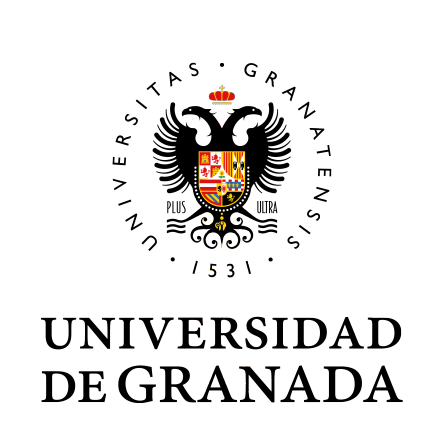
\includegraphics[scale=0.5]{img/ugr.png}\\

\textsc{\Large \asignatura{}\\[0.2cm]}
\textsc{GRADO EN INGENIERÍA INFORMÁTICA}\\[1cm]

\noindent\rule[-1ex]{\textwidth}{1pt}\\[1.5ex]
\textsc{{\Huge PRÁCTICA 1\\[0.5ex]}}
\textsc{{\Large Técnicas de Búsqueda\\}}
\noindent\rule[-1ex]{\textwidth}{2pt}\\[3.5ex]

\end{minipage}

\vspace{0.4cm}

\begin{minipage}{\textwidth}

\centering

\textbf{Autores}\\ {Vladislav Nikolov Vasilev}\\ {Carlos Núñez Molina}\\[2ex]
\textbf{Rama}\\ {Computación y Sistemas Inteligentes}\\[2ex]
\vspace{0.3cm}


\includegraphics[scale=0.3]{img/etsiit.jpeg}

\vspace{0.7cm}
\textsc{Escuela Técnica Superior de Ingenierías Informática y de Telecomunicación}\\
\vspace{1cm}
\textsc{Curso 2018-2019}
\end{minipage}
\end{titlepage}

\pagenumbering{arabic}
\tableofcontents
\thispagestyle{empty}				% No usar estilo en la pagina de indice

\newpage

\setlength{\parskip}{1em}

\section{\textsc{Descripción General de la Solución}}

El aspecto fundamental de la práctica es cómo elegir qué gemas coger y en qué orden. Hay en total 23
gemas por nivel, de las cuales solo se necesitan coger 9. Si se hacen los cálculos, hay
${23\choose 9} \cdot 9! = 296541907200$ combinaciones posibles. Este número es inabarcable para el
A*, sin importar la estrategia usada, por lo que no podemos usarlo para que resuelva el nivel desde
cero: hace falta simplificar el problema.

Para reducir el número de posibilidades se ha usado una estrategia de \textit{clustering}, técnica de
aprendizaje no supervisado. La heurística detrás de esto es la siguiente: si nos encontramos en un
\textit{cluster} (grupo) de gemas, al estar estas gemas todas juntas, generalmente será una buena idea
(un buen plan) coger todas las gemas del \textit{cluster} antes de irse a otro. Por tanto, hemos
transformado el problema de qué gemas coger y en qué orden al problema de qué \textit{clusters} de
gemas coger y en qué orden. Como el número de \textit{clusters} es mucho menor que el de gemas, este
problema sí que es abordable. Para generar los \textit{clusters} se ha usado un algoritmo llamado
\textit{DBSCAN}. Su funcionamiento (implementado) es el siguiente: se va iterando por todas las gemas
del nivel; si esa gema no pertenece a un \textit{cluster} y no hay otra gema de algún \textit{cluster}
cerca suya se crea un nuevo \textit{cluster} y se asigna a él; después se ve qué otras gemas sin
\textit{cluster} están cerca de ésta y se asignan al mismo \textit{cluster}. Una gema está cerca de
otra si su distancia Manhattan es menor o igual a un parámetro $\varepsilon$ del método. En la
práctica se ha usado $\varepsilon = 3$, que es el que genera mejores \textit{clusters}. Para elegir el
\textit{tour} (camino) a través de los \textit{clusters} se ha usado un simple algoritmo de
\textit{Branch}\&\textit{Bound}, que devuelve un camino a través de \textit{clusters} de forma que en
total se consigan el número de gemas necesarias para abandonar el nivel, siendo el camino elegido en
función de la distancia entre los \textit{clusters} y la ``dificultad'' de cada \textit{cluster} (el
número de rocas, muros y enemigos en el \textit{cluster} y cómo de alejadas están sus gemas).

De esta forma, esta es la estrategia fundamental usada en la resolución de la práctica: agrupar las
gemas en \textit{clusters} e ir yendo de un \textit{cluster} a otro hasta tener 9 gemas, en cuyo caso
se planifica para abandonar el nivel.

La integración del comportamiento reactivo y deliberativo, a grandes rasgos y en pseudocódigo, es la
siguiente:

\begin{algorithm}
\caption{Integración del comportamiento reactivo-deliberativo (I)}
\begin{algorithmic}[1]
\Procedure{act}{$ $}
\If{$primer\_turno$} \Comment{Esto se hace en el constructor}
	\State crearClusetrsYCircuitos()
	\State $cluster\_actual \gets 0$
	\State buscarPlan($cluster\_actual$)
\algstore{bkact}
\end{algorithmic}
\end{algorithm}

\begin{algorithm}[H]
\caption{Integración del comportamiento reactivo-deliberativo (II)}
\begin{algorithmic}[1]
\algrestore{bkact}
\EndIf
\State \Comment{Plan creado cuando el jugador puede o va a morir en próx. turnos}
\If{$plan\_no\_morir$.isEmpty()}
	\State \textbf{return} $plan\_no\_morir$.first()
\EndIf
\If{$num\_gems \geq 9$} \Comment{Dirigirse a la salida si se puede salir}
	\State buscarPlanAbandonarNivel()
\EndIf
\If{$busqueda\_no\_terminada$} \Comment{Búsqueda puede tardar múlt. turnos}
	\State seguirBuscandoPlan()
\EndIf
\If{$busqueda\_terminada$ \textbf{and} $camino\_no\_encontrado$}
	\State $hay\_que\_replanificar \gets $ true
	\If{$num\_gems < 9$}
		\State removeCluster($cluster\_actual$) \Comment{Eliminar \textit{cluster} y recrear circuito}
		\State crearClusterYCircuito() \Comment{porque el \textit{cluster} es inaccesible}
	\EndIf
\EndIf
\If{$hay\_que\_replanificar$}
	\State buscarPlan()
\EndIf
\If{$busqueda\_terminada$}
	\If{$plan\_vacio$}
		\State $cluster\_actual \gets cluster\_actual + 1$
		\State buscarPlan($cluster\_actual$)
	\Else
		\State $accion \gets plan$.first()
	\EndIf
\EndIf
\State \Comment{Parte reactiva: ver si ejecutar la acción del plan o no}
\If{$enemigos\_cercanos$ \textbf{or} $muerte\_por\_roca$}
	\State crearPlanNoMorir()
	\State \textbf{return} $plan\_no\_morir$.first()
\EndIf
\If{$jugador\_choca\_con\_roca\_cayendo$}
	\State \textbf{return} $quedarse\_quieto$
\EndIf
\State \textbf{return} $accion$
\EndProcedure
\end{algorithmic}
\end{algorithm}

\section{\textsc{Comportamiento Reactivo}}

\newpage

\section{\textsc{Comportamiento Deliberativo}}

Para la realización del comportamiento deliberativo se han implementado tres versiones del A*: una
que permite ir de una posición inicial a una final, una que permite ir de una posición inicial a
una final recogiendo las gemas de un \textit{cluster} y una parecida a la anterior pero sin posición
final. En las tres, aparte de las listas que utiliza el algoritmo, se ha añadido una lista de explorados
que contiene los nodos visitados y los expandidos para poder hacer una consulta rápida de qué nuevos
nodos expandir y cuáles no. La lista de nodos cerrados no se revisita, ya que la optimalidad no es lo más
importante en este caso al estar trabajando a nivel de \textit{cluster} y no de gemas. Como se valora
mucho la eficiencia en el tiempo, se ha modificado el A* para que las búsquedas se puedan ejecutar en
varios turnos, guardando la información internamente.

Se han usado 2 heurísticas distintas, una para el A* que busca un camino desde una casilla inicial a
otra final y otra para el A* que busca un camino que coja todas las gemas de un \textit{cluster}.

\begin{itemize}[label=\textbullet]
	\item \textbf{Heurística camino, \textit{getHeuristicDistance}}:
	Obtiene la longitud del camino (número de
	casillas de separación) que une ambas casillas, pudiendo atravesar rocas pero no muros. Si la
	casilla inicial y final difieren en su posición $x$ y su posición $y$, aumenta en 1 la distancia
	(ya que el agente tendrá que girar una vez como mínimo para llegar al destino). Debido a que
	puede atravesar las rocas (a diferencia del agente), esta es una heurística obtenida mediante un
	modelo relajado, con lo que es admisible y monótona.
	\item \textbf{Heurística gemas, \textit{getHeuristicGems}}:
	Crea un grafo donde las $n$ gemas dadas son 
	los $n$ nodos y escoge los $n-1$ lados más cortos de este grafo. El coste del lado entre la gema
	$a$ y $b$ se corresponde con el valor de la distancia entre $a$ y $b$, medida usando
	$getHeuristicDistance$.
	
	Esta heurística devuelve la suma de la distancia de la casilla inicial a la gema más cercana a
	esta, más la suma de los $n-1$ lados más cortos del grafo mencionado anteriormente, más la
	distancia de ir de la casilla final a su gema más cercana. La heurística sería admisible y
	monótona si se usara así, pero hemos decidido multiplicar esta suma por $\alpha = 2$, con lo que
	deja de ser admisible y monótona, a cambio de aproximar mejor la longitud real del camino, lo que
	hace que el A* tenga que explorar menos estados. Aunque no consiga la solución óptima de esta
	forma, hemos hecho pruebas y, de media, este camino no tiene más de 5 casillas de diferencia con
	el óptimo.
\end{itemize}

A continuación se procede a mostrar el pseudocódigo de la primera versión del A*, sobre la que se
comentarán brevemente las otras:

\begin{algorithm}[H]
\caption{Versión del A* para ir de un inicio a un final}
\begin{algorithmic}[1]
\Procedure{buscarPlan}{$inicio, fin, casillas\_ignorar$}
\State $plan \gets \varepsilon$
\State Inicializar variables y listas
\While{\textbf{not} $encontrado$ \textbf{and not} $lista\_abiertos$.empty() \textbf{and not} $timeout$}
	\State Comprobar si se ha producido $timeout$
	\State $nodo \gets lista\_abiertos$.getRemoveFirst()
	\If{$nodo$.posicion() $ = fin$}
		\State \textbf{$encontrado \gets $ true}
	\Else{}
		$vecinos \gets $ obtenerVecinos($nodo$.posicion())
		\ForEach{$vecino \in vecinos$}
			\If{posicionValida($vecino$) \textbf{and} $vecino \notin casillas\_ignorar$}
				\State Generar costes e informacion para el siguiente nodo
				\If{$vecino$ produce caída de roca}
					\State Simular caída de rocas y generar nueva información
				\EndIf
				\If{ $vecino \notin lista\_explorados$}
					\State $lista\_abiertos$.add(siguiente nodo)
					\State $lista\_explorados$.add(siguiente nodo)
				\EndIf{}
			\EndIf{}
		\EndFor
	\EndIf
	
	\State $lista\_cerrados$.addFirst($nodo$)
\EndWhile
\If{$timeout$}
	\State Guardar información
	\State \textbf{return}
\EndIf
\If{$encontrado$}
	\State $plan \gets$ procesarPlan($lista\_cerrados$.getFirst())
\EndIf
\State \textbf{return} $plan$
\EndProcedure
\end{algorithmic}
\end{algorithm}

Sobre esta implementación de la primera versión se tienen que realizar muy pocas modidicaciones para
llegar a las otras versiones. En el caso de la segunda, hay que pasarle una lista de gemas que coger,
comprobar en la línea 7 también si se han cogido todas las gemas y usar una u otra heurística al generar
un nuevo nodo. En el caso de la tercer versión, respecto a la anterior, no hay que pasarle una posición
final y en la línea 7 solo comprobar si se han cogido todas las gemas de la lista.

\end{document}

